\chapter{Технологический раздел}

В данном разделе будут выбраны СУБД, средства реализации приложения, а также спроектирован пользовательский интерфейс.

\section{Выбор СУБД}

В данной работе предусмотрена четкая структурированность хранимых данных, что позволяет использовать реляционную базу данных, являющуюся удобной и наиболее широко используемой. Данный тип БД обеспечивает хранение данных в виде двумерных таблиц, столбцы которых определяют множество используемых значений, а строки -- конкретные записи базы данных. 

Среди самых распространенных систем управления базами данных можно выделить Microsoft SQL Server \cite{ms_sql}, PostgreSQL \cite{postgresql} и  Oracle \cite{oracle}. При реализации будет использован PostgreSQL, так как он уже использовался в ранее изученном курсе.

\section{Средства реализации}

В качестве используемого языка программирования выбрана Java \cite{java}, так как:
\begin{itemize}
	\item данный язык является объектно-ориентированным, позволяя использовать наследование, интерфейсы, абстракции и т.~д.;
	\item имеет JDBC \cite{jdbc} -- API для выполнения SQL-запросов к базам данных.
\end{itemize}

В качестве среды разработки используется IntelliJ IDEA \cite{intellij_idea}, поскольку данная программа:
\begin{itemize}
	\item имеет удобный интерфейс взаимодействия и подключения используемых зависимостей;
	\item предоставляет возможности тестирования и запуска написанного приложения с определенными файлами конфигурации.
\end{itemize}

\section{Реализованные функции}

Для спроектированного триггера была написана соответствующая функция с помощью PL/pgSQL \cite{plpgsql} -- процедурного расширения языка SQL, используемого в СУБД PostgreSQL. Код функции представлен в листинге \ref{trigger_code}.

\captionsetup{singlelinecheck = false, justification=raggedright}
\begin{lstlisting}[language=sql, caption=Реализация триггера AFTER на добавление заявки, label=trigger_code]
create or replace function checkBanWords()
returns trigger as 
$$
declare 
	banWords text ARRAY;
begin 
	banWords := ARRAY(select '%' || word || '%' from sosedushka_db.ban);
	if new.title like any (banWords) or new.explanation like any (banWords)
	then
		raise notice 'Bad words existing!';
		update sosedushka_db.request set status='BANNED' where id=new.id;
		return null;
	else
		return new;
	end if;
end
$$
language plpgsql

create trigger newRequest
after insert 
on sosedushka_db.request 
for each row 
execute function checkBanWords()
\end{lstlisting}
\captionsetup{singlelinecheck = false, justification=centering}

\section{Интерфейс приложения}

Для работы с базой данных был разработан интерфейс взаимодействия в виде telegram-бота. На рисунках \ref{personalize}-\ref{administrator} представлены примеры персонализации, взаимодействия с системой оформителя, исполнителя и администратора. 

\begin{figure}[H]
	\begin{center}
		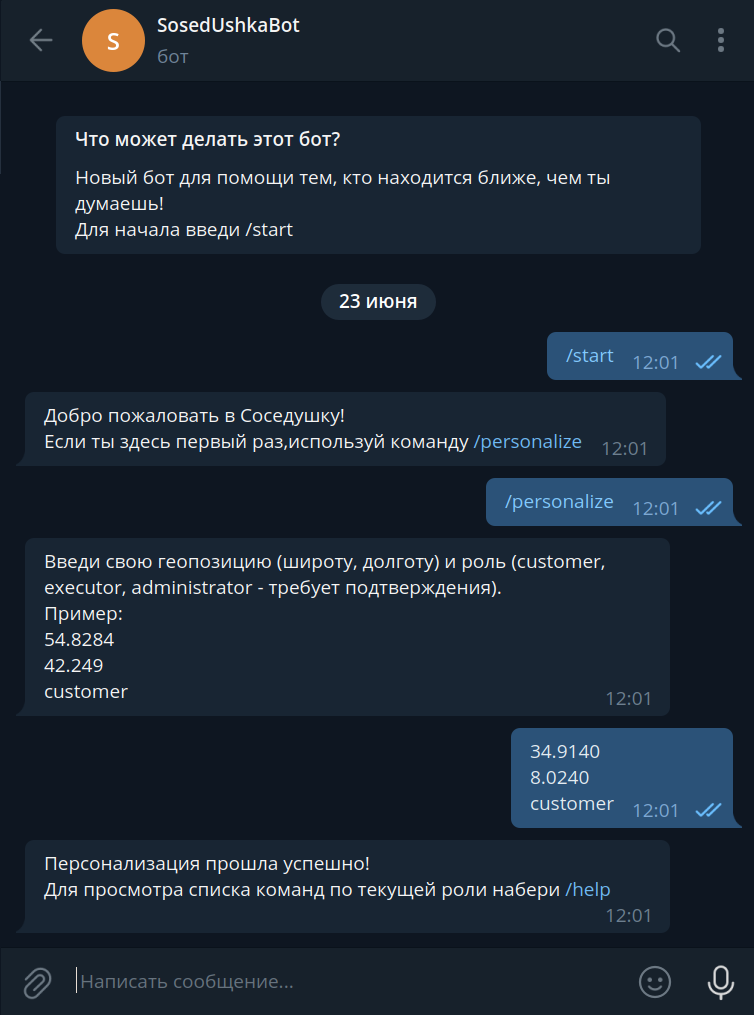
\includegraphics[scale=0.3]{assets/personalize.png}
	\end{center}
	\caption{Интерфейс персонализации}
	\label{personalize}
\end{figure}

\begin{figure}[H]
	\begin{center}
		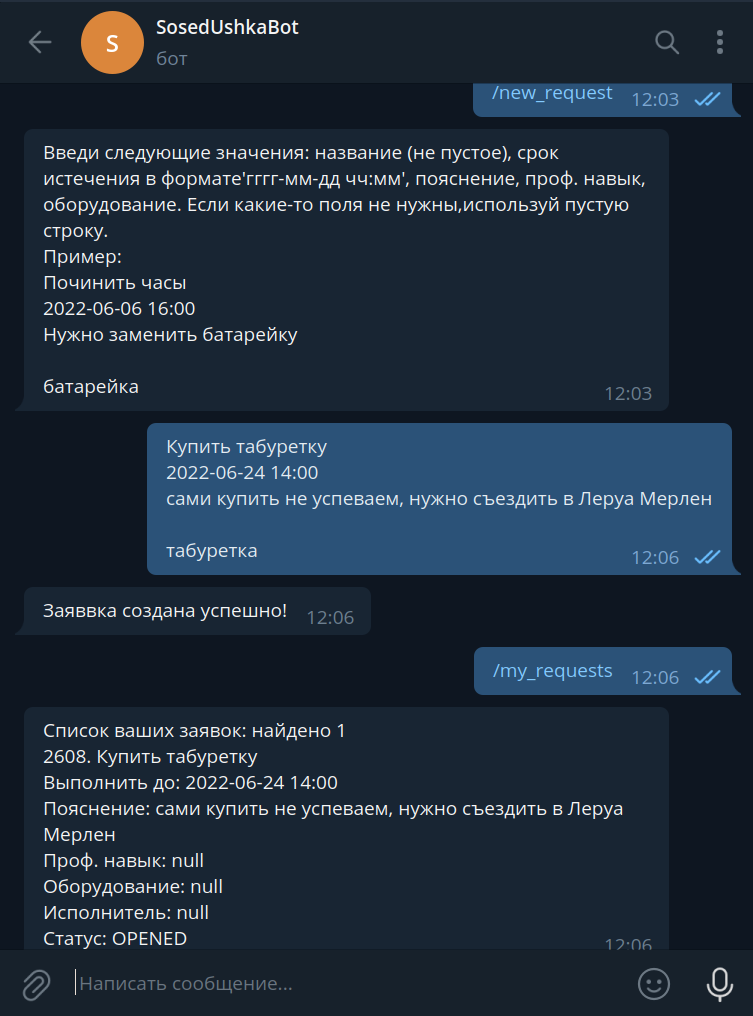
\includegraphics[scale=0.3]{assets/customer.png}
	\end{center}
	\caption{Интерфейс оформителя}
	\label{customer}
\end{figure}

\begin{figure}[H]
	\begin{center}
		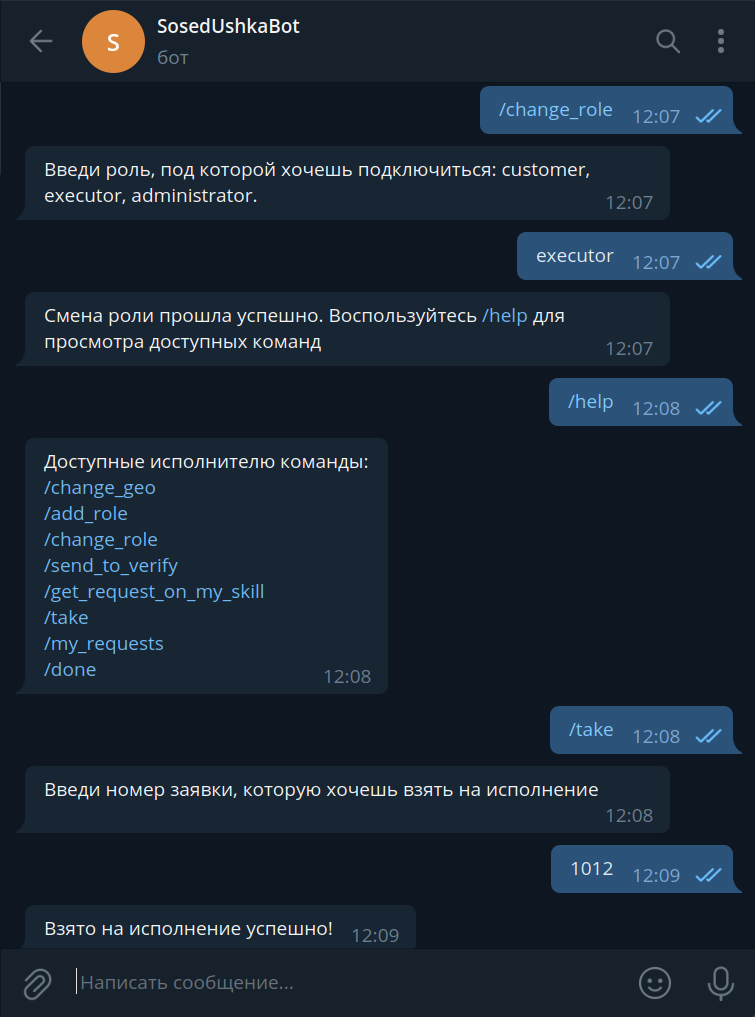
\includegraphics[scale=0.3]{assets/executor.png}
	\end{center}
	\caption{Интерфейс исполнителя}
	\label{executor}
\end{figure}

\begin{figure}[H]
	\begin{center}
		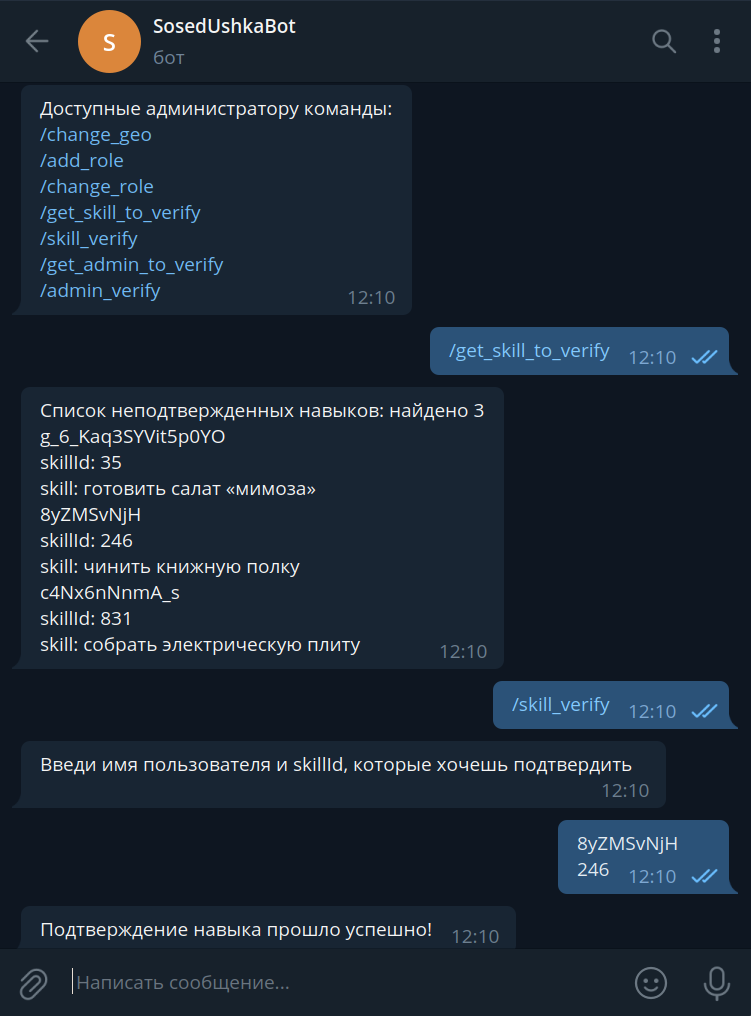
\includegraphics[scale=0.3]{assets/administrator.png}
	\end{center}
	\caption{Интерфейс администратора}
	\label{administrator}
\end{figure}

\section{Вывод из раздела}

В данном разделе был сделан выбор СУБД и средств реализации, а также реализован триггер и пользовательский интерфейс.